% !TEX root = ../../document.tex

\documentclass{subfiles}

\begin{document}

  \chapter{Algoritmo PageRank}
  \label{chap:pagerank}

    \section{Introducción}
    \label{sec:pagerank_intro}

      \paragraph{}
      El algoritmo \emph{PageRank} fue nombrado por primera vez en el trabajo \emph{The PageRank citation ranking: Bringing order to the web} \cite{page1999pagerank} publicado por \emph{Larry Page} y \emph{Sergey Brin}. La motivación del mismo fue tratar de realizar un \emph{ranking de importancia} (o relevancia) sobre los nodos de un \emph{grafo dirigido no ponderado} de tal manera que este esté basado únicamente en la estructura de dicho grafo.

      \paragraph{}
      La motivación de dicho trabajo fue la de tratar de mejorar el ranking de resultados del buscador de sitios web \emph{Google} en que estaban trabajando. Hasta la publicación de dicho trabajo, los sistemas de búsqueda se basaban en heurísticas como el número de ocurrencias de la palabra clave sobre la cual se basaba la búsqueda o el número de enlaces hacia dicha página.

      \paragraph{}
      Sin embargo, los rankings basados en este tipo de estrategias podían ser fácilmente manipulables con el fin de tratar de conseguir posicionarse en las primeras posiciones del sistema de búsqueda. Por ejemplo, una página web que se basara en la repetición de la misma palabra muchas veces, entonces aparecería en primer lugar en rankings basados en el número de ocurrencias para dicha palabra clave. En el caso de rankings basados en el número de enlac hacia dicha página, tampoco sería complejo manipular el resultado creando un número elevado de páginas web que contuvieran links hacia la página para la cual se pretende mejorar su posicionamiento.

      \paragraph{}
      La solución propuesta por \emph{Page} y \emph{Brin} para tratar de solucionar dicha problemática se basa en la generación de un ranking sobre los sitios web basado en la estructura del grafo subyacente, de tal manera que los vértices (sitios web) sobre los cuales existan aristas (enlaces) que provengan de otros vértices relevantes, tendrán una puntuación mayor que la de vértices que cuyo subconjunto de aristas los relacione con otros vértices menos relevantes.

      \paragraph{}
      La idea en que se basa el ranking se refiere por tanto a que los sitios web a los cuales se puede acceder a partir de otros sitios web considerados como importantes, entonces deberan encontrarse en primeras posiciones. Esta idea se extiende de manera inductiva sobre todos los vértices del grafo, puesto que tal y como veremos en las siguientes secciones converge hacia un estado estable (o \emph{distribución estacionaria} desde el punto de vista estadístico)

      \paragraph{}
      Para tratar de facilitar la comprensión acerca de esta idea a continuación se expone un ejemplo: Supongamos que en una red social como \emph{Twitter} (la cual se puede entender como un conjunto de usuarios que se relacionan entre si mediante relaciones de seguimiento, por lo que se puede ver como un grafo dirigido no poderado donde el conjunto de usuarios se refiere a los vértices y el conjunto de relaciones de seguimiento con las aristas) un usuario habitual (el cual no tiene un número elevado de seguidores) comienza a seguir a un antiguo amigo de la universidad, el cual tampoco tiene un gran número de seguidores.

      \paragraph{}
      La red social \emph{Twitter} envía una notificación a todos seguidores del usuario indicando que este ha empezado a seguir a su amigo de la universidad. Puesto que su número de seguidores es bajo dicha acción no tendrá una gran relevancia y muy probablemente nadie más comience a seguir al amigo de la universidad. Sin embargo, supongamos que nuestro usuario, en lugar de tener un conjunto reducido de seguidores, es una persona influyente en la red social, a la cual siguen millones de personas, entonces la notificación del nuevo seguimiento le llegará a muchos más usuarios y probablemente el amigo de la universidad verá como su número de seguidores aumenta notablemente.

      \paragraph{}
      A grandes rasgos, esta es la idea en que se basa el algoritmo \emph{PageRank}, es decir, la puntuación de un vértice del grafo se basa en la relevancia de los vértices que contienen aristas que apuntan hacia el propio vértice.

      \paragraph{}
      La idea inicial del algoritmo \emph{PageRank} era la de realizar un ranking basado en la estructura del grafo de la web (\emph{Web Graph}), sin embargo, tal y como se verá a lo largo del capítulo, los conceptos matemáticos en que se basa dicho ranking son extrapolables a cualquier entorno que se pueda representar a partir de una red o grafo. En el trabajo \emph{PageRank beyond the Web}\cite{gleich2015pagerank} \emph{Gleich} realiza un estudio acerca de los distintos entornos sobre los cuales se han aplicado estas ideas.

      \paragraph{}
      Entre otros, se han realizado trabajos sobre los cuales se ha aplicado el algoritmo \emph{PageRank} en áreas tan dispares como la Biología, para analizar las células más importantes a partir de las interrelaciones entre ellas. También se ha aplicado en el sector de la neurociencia por razones similares. En el caso de la literatura, se ha aplicado sobre el grafo generado a partir del sistema de citaciones de artículos de investigación. Otros ámbitos de aplicación han sido sistemas de planificación de tareas o incluso estudios acerca de resultados en deportes, para conocer los encuentros más relevantes.


      \paragraph{}
      [TODO hablar acerca de cómo se va a organizar el resto del capítulo]


    \section{Paseos Aleatorios}
    \label{sec:random_walks}

      \paragraph{}
      En esta sección se trata el concepto de \emph{Paseos Aleatorios}, el cual está intimamente relacionado con el algoritmo \emph{PageRank}. Para el desarrollo de esta sección se ha utilizado como herramienta bibliográfica el libro \emph{Randomized algorithms} \cite{motwani2010randomized} de \emph{Motwani} y \emph{Raghavan}, concretamente se ha prestado especial atención al \emph{capítulo 6: Markov Chains and Random Walks}. El resto de la sección se basará en la descripción de propiedades relacionadas con \emph{Paseos Aleatorios} para finalizar ilustrando la relacion de estos con \emph{PageRank}

      \paragraph{}
      Lo primero que haremos será describir en qué consiste un \emph{Paseo Aleatorio}. Para ello nos referiremos al grafo $G=(V,E)$ dirigido y no ponderado, el cual esta compuesto por $n = card(V)$ vértices y $m=card(E)$ aristas. Un paseo aleatorio se refiere entonces a un camino de longitud $l$ con origen en el vértice $v_{i_1}$ y final en $v_{i_l}$. Para que dicho camino constituya un paseo aleatorio, cada paso debe haber sido generado seleccionando de manera uniforme el siguiente vértice a visitar de entre los adyacentes al vértice actual. Nótese que este comportamiento puede ser visto como el promedio del modo en que los usuarios navegan por internet, de tal manera que acceden a páginas web mediante los enlaces que encuentran en la página que están visualizando. A continuación se describen las \emph{Cadenas de Markov} por su relación como herramienta de estudio para los paseos aleatorios.


      \subsection{Cadenas de Markov}
      \label{sec:markov_chains}

        \paragraph{}
        Para el estudio de paseos aleatorios, es apropiado utilizar la abstracción conocida como \emph{Cadenas de Markov}, las cuales están intimamente relacionadas con el concepto de grafo y máquina de estados. Una \emph{Cadena de Markov} $M$ se define como un proceso estocástico que consta de $n$ posibles estados, los cuales tienen asociadas un conjunto de probabilidades denotadas como $p_{ij}=\frac{A_{ij}}{d^-(i)}$ para indicar la probabilidad con la cual se pasará del estado $i$ al estado $j$.

        \paragraph{}
        Dichas probabilidades se pueden representar de manera matricial sobre una matriz de transiciones $P$ de tamaño $n*n$, de tal manera que la posición $(i,j)$ contenga el valor $p_{ij}$ construido tal y como se indica en el párrafo anterior. Notese por tanto, que $\sum_{j}p_{ij}=1$ para que la distribución de probabilidades sea válida, es decir, la suma de probabilidades para las transiciones sobre cada estado deben sumar $1$.

        \paragraph{}
        Supongase que se realiza un paseo aleatorio sobre la \emph{Cadena de Markov} $M$ cuya longitud $l$ es muy elevada ($l \gg n^2$), entonces, es fácil intuir que se visitará más de una vez cada estado. Sin embargo, el ratio de veces que se visitará cada estado muy probablemente no se distribuirá de manera uniforme, sino que habrá estados que serán visitados muchas más veces que otros. Esto depende en gran medida de la matriz de transicciones $P$. A la distribución de probabilidad generada sobre el ratio de visitas sobre cada nodo tras aplicar un paseo aleatorio de longitud elevada se le conoce como \emph{distribución estacionaria} y se denota como $\pi$.

        \begin{figure}
          \centering
          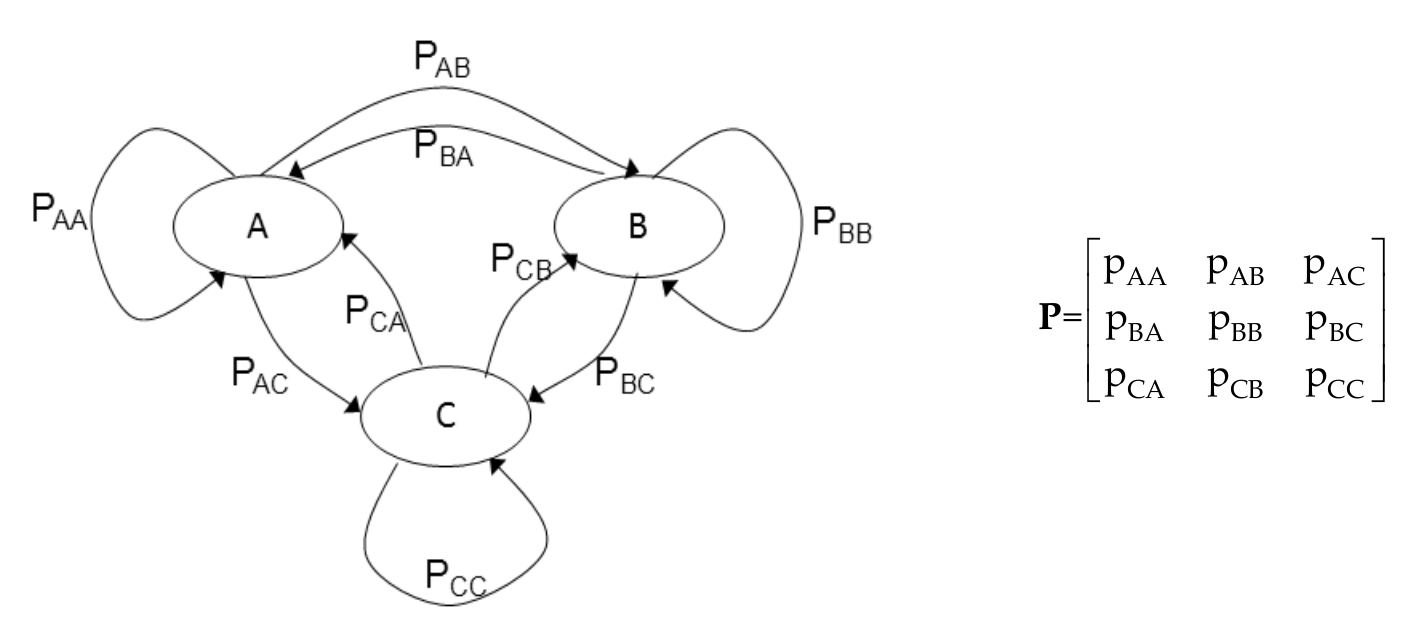
\includegraphics[width=0.6\textwidth]{markov-chain-example}
          \caption{Ejemplo de \emph{Cadena de Markov}. (Extraido de \cite{sanchez2012wireless})}
          \label{img:markov_chain_example}
        \end{figure}

        \paragraph{}
        En la figura \ref{img:markov_chain_example} (Extraido de \cite{sanchez2012wireless}) se muestra una cadena de markov constituida por 3 estados, tando en su forma de grafo dirigido como de forma matricial.

        \paragraph{}
        La distribución estacionaria $\pi$ existe siempre que la \emph{Cadena de Markov} $M$ permita que a partir de un determinado estado $i$, se pueda llegar al menos a otro estado $j$. La razón se debe a que si se llega al estado $i$ y este no contiene más posibles estados de salida, entonces el resto de épocas se seguirá en el mismo estado. A los estados que poseen esta característica se los denomina sumideros. La segunda restricción para que se pueda calcular la distrbución estacionaria $\pi$ es que la matriz de transiciones $P$ no debe ser periodica, es decir, no debe contener ciclos de probabilidad constante sobre los cuales el paseo aleatorio se quedaría iterando de manera indefinida.

        \paragraph{}
        Las definiciones descritas en este apartado se pueden extender de manera trivial al caso de grafos dirigidos sin más que utilizar cada vértice del grafo como un estado y construir la matriz $P$ de tal manera que $p_{ij}=\frac{A_{ij}}{d^-(i)}$ donde $d^-(i)$ representa el cardinal de aristas cuyo origen es el vértice $i$. Tal y como se verá posteriormente, el vector $\pi$ se corresponde con el resultado obtenido por el algoritmo \emph{PageRank} sobre una matriz $P$ de transicciones modificada.

      \subsection{Matriz Laplaciana de Paseos Aleatorios Normalizada}
      \label{sec:random_walk_normalized_laplacian_matrix}

        \paragraph{}
        En la sección \ref{sec:laplacian_matrix} se habló sobre la \emph{Matriz Laplacina}, la cual es una estrategia de representación, que ilustra distintas propiedades sobre el grafo subyacente. En este caso se describe una variación de la misma que es más apropiada para problemas relacionados con \emph{Paseos Aleatorios}. Esta se denota como $L^{{{\text{rw}}}}$ y se denomina \emph{Matriz Laplaciana de Paseos Aleatorios Normalizada}. La estrategia de construcción de la misma se indica en la ecuación \eqref{eq:random_walk_normalized_laplacian_matrix}. Esto consiste en asignar a la posición $(i,j)$ el opuesto de la probabilidad de transicción del vértice $i$ al vértice $j$. Además, en la diagonal $(i,i)$ se asigna el valor $1$ cuando el grado del vértice es mayor que $0$.

        \begin{equation}
        \label{eq:random_walk_normalized_laplacian_matrix}
          L_{{i,j}}^{{{\text{rw}}}}:={
          \begin{cases}
            1&{\mbox{if}}\ i=j\ {\mbox{and}}\ d(v_{i})\neq 0\\
            -{P_{ij}}&{\mbox{if}}\ i\neq j\ {\mbox{and}}\ v_{i}{\mbox{ is adjacent to }}v_{j}\\
            0&{\mbox{otherwise}}.
          \end{cases}}
        \end{equation}


      \paragraph{}
      Una vez descritos los \emph{Paseos Aleatorios}, junto con las \emph{Cadenas de Markov} y la \emph{Matriz Laplaciana de Paseos Aleatorios Normalizada}, ya se está en condiciones suficientes como para describir de manera formal el \emph{PageRank} de un determinado grafo, que se realizará en la siguiente sección. Para ello, se indicarán las dificultades que surgen sobre este problema en grafos reales, así como las soluciones utilizadas para poder hacer frente a estas.

    \section{Definición Formal}
    \label{sec:pagerank_formal_definition}

      \paragraph{}
      Se define el \emph{PageRank} como la \emph{distribución estacionaria} $\pi$ de un determinado grafo dirigido no ponderado $G$ sobre el cual, la matriz de transicciones $P$, ha sido ligeramente modificada. Tal y como se ha visto en la sección anterior, la \emph{distribución estacionaria} consiste en la probabilidad de encontrarse en el estado $i$ durante un paseo aletorio de longitud elevada sobre la \emph{Cadena de Markov} $M$. Tal y como se ha indicado, para que una cadena de markov sea válida, entonces no deben existir estados \emph{sumideros} (no tienen posibles estados próximos).

      \paragraph{}
      Por estas razones, obtener la \emph{distribución estacionaria} de un grafo $G$, este no debe contener vértices \emph{sumideros}. La solución que proponen \emph{Page} y \emph{Brin} en \cite{page1999pagerank} para encontrar la \emph{distribución estacionaria} o \emph{PageRank} del grafo generado por los enlaces de la web (\emph{Web Graph}) es añadir un determinado índice de probabilidad sobre el cual los usuarios dejan de seguir los enlaces entre páginas web para acceder a otra distinta introducciendo la URL directamente. El apoyo en esta estrategia soluciona por tanto el problema de los vértices \emph{sumidero}, además de asemejarse en un mayor grado al comportamiento real de un usario que navega por internet.

      \paragraph{}
      En \cite{page1999pagerank} \emph{Page} y \emph{Brin} proponen la modificación de la matriz de transiciones $P$ para la adaptación descrita en el párrafo superior, la cual se indica en la ecuación \eqref{eq:pagerank_transition_matrix}. De esta manera, se representa la situación en la cual un determinado usuario que llega a una página web sin enlaces hacia otras (\emph{sumidero}), accede a otra seleccionada de manera uniforme (esto se modeliza mediante el vector $v$ construido de tal manera que  $v_{i} = \frac{1}{n}, \ \forall i \in [1,n]$). Además, se añade un determinado índice $\beta$, que se corresponde con la probabilidad de que el usuario continue seleccionando enlaces en la página actual o ,por contra, acceda a otra seleccionandola de manera uniforme. Típicamente el valor $\beta$ se fija a $0.85$, sin embargo, admite cualquier valor contenido en el intervalo $[0,1]$.

      \begin{equation}
      \label{eq:pagerank_transition_matrix}
        p'_{ij} =
        \begin{cases}
          \beta * \frac{A_{ij}}{d^-(i)} + (1- \beta) * v_{i} & \mbox{if} \ d^-(i) \neq 0 \\
          v_{i}&\mbox{otherwise}
        \end{cases}
      \end{equation}

      \paragraph{}
      Tal y como se ha indicado anteriormente, el vector $v$ representa la distribución de probabilidad referida a los saltos que un usuario lleva a cabo entre sitios web sin tener en cuenta los enlaces del sitio web actual. En el párrafo anterior se ha indicado que este vector es construido siguiendo una distribución uniforme, por tanto, esto puede ser visto de tal manera que la probabilidad de saltar de un sitio web a otro es la misma. Sin embargo, dicha acción podría seguir una distribución de probabilidad distinta dependiendo de cada usuario de la red. Por tanto, en \cite{page1999pagerank} se habla de \emph{PageRank Personalizado} cuando el vector $v$ sigue una distribución de probabilidad distinta de la uniforme (desviada hacia los sitios web a los que más accede el usuario).

      \paragraph{}
      En el trabajo \emph{Topic-sensitive pagerank} \cite{haveliwala2002topic} \emph{Haveliwala} propone la generación de 16 \emph{distribuciones estacionarias} (\emph{PageRanks}) distintas mediante la personalización del vector $v$, para después realizar una combinación de estas y así conseguir que el ranking final sea personalizado.

      \paragraph{}
      Una vez descritas las transformaciones necesarias a realizar sobre la matriz de transiciones $P$ para que esta se adapte a la estructura de grafos con vértices \emph{sumidero}, y que además emule de manera más apropiada el comportamiento de un determinado usuario sobre el grafo de la web (\emph{Web Graph}), lo siguiente es explicar cómo se puede obtener la \emph{distribución estacionaria} o \emph{PageRank} del grafo. Para ello, a continuación se describe el \emph{Teorema de Perron–Frobenius}, que aporta una idea acerca de la manera en que se calcula, además de asegurar la convergencia de la matriz de transiciones hacia un estado estacionario del vector $\pi$.

      \subsection{Teorema de Perron–Frobenius}
      \label{sec:perron_frobenius_theorem}

        \paragraph{}
        El \emph{teorema de Perron–Frobenius} se refiere a la existencia de un \textbf{único} \emph{vector propio} (\emph{eigenvector}) para las matrices cuadradas reales positivas. Dicha descripción ha sido extraida del documento \emph{Notes on the perron-frobenius theory of nonnegative matrices} \cite{boyle2005notes} de \emph{Boyle} (profesor de matemáticas de la \emph{Universidad de Marylan}). En primer lugar es necesario describir los conceptos de \emph{vector propio} como de \emph{matriz cuadrada real positiva} para después ver que la \emph{distribución estacionaria} y la \emph{matriz de transiciones} referidos a una \emph{Cadena de Markov} $M$ pueden ser vistos de esta manera.

        \paragraph{}
        Una \emph{matriz cuadrada real positiva} $A$ es aquella formada por $n$ filas y $n$ columnas ($n*n$ celdas) para las cuales $\forall i,j \in [1,n]$ se cumple que $A_{ij} \in \mathbb{R} \geq 0$. Tal y como se puede apreciar, la \emph{matriz de transiciones modificada} $P'$ del grafo $G$ cumple esta propiedad ya que $\forall i,j \in [1,n] \ P'_{ij} \in [0,1]$.

        \paragraph{}
        En cuanto al concepto de \emph{vector propio} $\lambda$ de un matriz, se refiere a un vector de $n$ columnas ($1*n$) tal que cuando es multiplado por una determinada matriz $A$, el resultado sigue siendo el mismo. Es decir, se cumple que $\lambda = \lambda * A$. Notese por tanto, que esta idea es equivalente a la \emph{distribución estacionaria} desde el punto de vista de llegar a un estado estable.

        \paragraph{}
        El teorema de \emph{teorema de Perron–Frobenius} asegura por tanto, que para una \emph{matriz cuadrada real positiva} $A$ tan solo existe un único \emph{vector propio} $\lambda$ y el conjunto de valores de este se es estrictamente positivo, es decir, $\forall i \in [1,n] \ \lambda_i \geq 0$. La demostración de dicho teorema puede encontrarse en \cite{boyle2005notes}.

        \paragraph{}
        Además, en el caso de que la matriz $A$ haya sido normalizada por columna, es decir, se cumpla que $\forall i \in [1,n] \ \sum_j A_{ij} = 1$, entonces el autovector $\lambda$ también seguirá la propiedad de normalización ($\sum_i \lambda_i = 1$). Gracias a este resultado es posible calcular la \emph{distribución estacionaria} $\pi$ de una \emph{Cadena de Markov} como el \emph{vector propio} de su matriz de transiciones.

      \paragraph{}
      Una vez descrito el \emph{teorema de Perron–Frobenius} ya se está en condiciones suficientes para describir las distintas alternativas para calcular el \emph{PageRank} de un determinado grafo, el cual se calcula tal y como se ha indicado en esta sección, encontrando el \emph{vector propio} de la matriz de transición modificada de la cadena de markov. Las distintas estrategias para obtener este resultado se describen en la siguiente sección.

    \section{Algoritmo Básico}
    \label{sec:pagerank_algorithm}

      \paragraph{}
      En esta sección se describe el método para obtener el vector \emph{PageRank} sobre un determinado grafo $G$. Para ello, es necesario fijar 3 parámetros los cuales se indican a continuación:
      \begin{itemize}
        \item Matriz de Adjacencia $A$, que a partir de la cual se obtiene la estructura del grafo (Se habló de ella en la sección \ref{sec:adjacency_matrix}).
        \item El valor de probabilidad $\beta$ de seguir el paseo aleatorio a partir de la distribución del vértice actual (el cual se comentó en la sección anterior).
        \item El vector de personalización $v$ referido a la distribución de probabilidad de los saltos aleatorios entre vértices (también se habló en la sección anterior).
      \end{itemize}



      \paragraph{}
      Para calcular el \emph{vector propio} $\lambda$ existen distintas estrategias matemáticas. En esta sección se habla de dos estrategias, la primera de ellas basada en la resolución de un sistema de ecuaciones lineales mientras que la segunda se basa en acercamiento a la solución de manera iterativa. Tal y como se verá a continuación, la estrategia algebraica conlleva un coste computacional muy elevado, por lo que no es admisible sobre grafos de tamaño masivo. En estos casos se utiliza la estrategia iterativa u otras alternativas aproximadas de las cuales se hablará en la sección \ref{sec:pagerank_algorithm_approximated}.


      \subsection{Estrategia Algebraica}
      \label{sec:pagerank_algorithm_algebraic}

        \paragraph{}
        La idea de la estrategia algebraica se refiere a la búsqueda del vector $\lambda$ que resuelva la ecuación $\lambda = \lambda * P'$ como un sistema de ecuaciones lineales. Esto se puede llevar a cabo siguiendo el desarrollo de la ecuación \eqref{eq:pagerank_algorithm_algebraic_1}. Nótese que para ello no se utiliza la \emph{matriz de transiciones modificada} $P'$ explicitamente. En su lugar, esta es representada implicitamente a partir de las operaciones de \eqref{eq:pagerank_algorithm_algebraic_2} y \eqref{eq:pagerank_algorithm_algebraic_3}.

        \paragraph{}
        Para entender estas ecuaciones, lo primero es indicar la notación que se ha utilizado así como la interpretación de algunas operaciones: Se utiliza el símbolo $\boldsymbol{1}$ para denotar el vector columna de tamaño $n$ formado por $1$'s en todas sus posiciones. El símbolo $\boldsymbol{I}$ representa la matriz identidad ($1$'s en la diagonal y $0$'s en el resto) de tamaño $n$. El símbolo $d^-$ representa un vector columna de tamaño $n$ que representa en su posición $j$ el cardinal de aristas cuyo origen es el vértice $j$. Esto puede ser visto de la siguiente manera: $\forall j \in [1,n] \ \sum_i A_{ij} = d^{-}_{j}$. A nivel de operaciones es necesario resaltar el caso de la división $\frac{A}{d^-}$ por su carácter matricial. Esta se lleva a cabo realizando la división elemento a elemento por columnas.

        \begin{align}
          \label{eq:pagerank_algorithm_algebraic_1}
          \lambda =& \lambda * P' \\
          \label{eq:pagerank_algorithm_algebraic_2}
                  =& \beta * \lambda * \frac{A}{d^-} + \frac{1-\beta}{n}*\boldsymbol{1} \\
          \label{eq:pagerank_algorithm_algebraic_3}
                  =& \bigg(\boldsymbol{I} - \beta * \frac{A}{d^-}\bigg)^{-1} * \frac{1-\beta}{n}*\boldsymbol{1}
        \end{align}

        \paragraph{}
        A partir de las operaciones descritas en la ecuación \eqref{eq:pagerank_algorithm_algebraic_3}, se obtiene por tanto el \emph{vector propio} $\lambda$, que en este caso se refiere a la \emph{distribución estacionaria} de la \emph{cadena de markov} descrita por la matriz de transiciones modificada $P'$, por lo que es equivalente al vector \emph{PageRank}. Sin embargo, el calculo del vector \emph{PageRank} siguiendo esta estrategia conlleva un elevado coste computacional derivado de la necesidad de invertir una matriz de tamaño $n*n$, algo inadmisible para grafos de tamaño masivo. 

      \subsection{Estrategia Iterativa}
      \label{sec:pagerank_algorithm_iterative}

        \paragraph{}
        [TODO]

        \paragraph{}
        A partir de los tres parámetros de entrada $(A, \beta, v)$ se calcula la \emph{matriz de transiciones modificada} $P'$ siguiendo la definición de la ecuación \eqref{eq:pagerank_transition_matrix} y una vez obtenida dicha matriz se está en condiciones de calcular el vector \emph{PageRank} siguiendo la idea del \emph{vector propio} único expuesta en la sección anterior.


        \paragraph{}
        [TODO ]

    \section{Soluciones Aproximadas}
    \label{sec:pagerank_algorithm_approximated}

      \paragraph{}
      [TODO ]

      \section{Variantes}
      \label{sec:pagerank_variants}

        \paragraph{}
        [TODO ]

        \subsection{SymRank}
        \label{sec:symrank}

          \paragraph{}
          [TODO]

        \subsection{HITS}
        \label{sec:hits}

          \paragraph{}
          [TODO]

        \subsection{SALSA}
        \label{sec:salsa}

          \paragraph{}
          [TODO]

    \section{Conclusiones}
    \label{sec:pagerank_conclusions}

      \paragraph{}
      [TODO]

\end{document}
